\documentclass{beamer}
\usepackage{../tut-slides}
\usepackage{../mathoperatorsAuD}

\usepackage{csquotes}
\usepackage{cancel}

\usepackage{amsmath,amssymb}

\usepackage{tikz}
\usetikzlibrary{positioning,automata, matrix, trees}
\usetikzlibrary{calc,positioning,backgrounds,arrows.meta}
\usetikzlibrary{patterns,snakes}
\usepackage{forest}


\usepackage{booktabs}
\usepackage{tabularx}
\usepackage{tabu}
\newcommand*\head{\rowfont{\bfseries}}
\newcommand*{\tw}{\rowfont{\ttfamily}}

\renewcommand{\tabularxcolumn}[1]{>{\hspace{0pt}}m{#1}}

\usepackage{listings}
\lstset{ 
	basicstyle=\footnotesize\ttfamily,        % the size of the fonts that are used for the code
	breakatwhitespace=false,         % sets if automatic breaks should only happen at whitespace
	breaklines=true,                 % sets automatic line breaking
	commentstyle=\itshape,    	     % comment style
	escapeinside={\%*}{*)},          % if you want to add LaTeX within your code
	extendedchars=true,              % lets you use non-ASCII characters; for 8-bits encodings only, does not work with UTF-8
	firstnumber=1,                % start line enumeration with line 1000
	frame=none,
	keywordstyle=\bfseries,       % keyword style
	morekeywords={}, 
	language=C,                 % the language of the code
	numbers=left,                    % where to put the line-numbers; possible: (none, left, right)
	numbersep=5pt,                   % how far the line-numbers are from the code
	numberstyle=\tiny\color{cdgray!50}, % the style that is used for the line-numbers
	rulecolor=\color{cddarkblue}, 
	tabsize=2,	                   % sets default tabsize to 2 spaces
}
\lstdefinestyle{am0}{ 
	basicstyle=\footnotesize\ttfamily,        % the size of the fonts that are used for the code
	breakatwhitespace=false,         % sets if automatic breaks should only happen at whitespace
	breaklines=true,                 % sets automatic line breaking
	commentstyle=\color{cdgray},    	     % comment style
	escapeinside={(*@}{@*)},          % if you want to add LaTeX within your code
	extendedchars=true,              % lets you use non-ASCII characters; for 8-bits encodings only, does not work with UTF-8
	firstnumber=1,                % start line enumeration with line 1000
	frame=none,
	keywordstyle=\bfseries,       % keyword style
	morekeywords={READ,LOAD,GT,JMC,STORE,JMP,WRITE}, 
%	language=AM0,                 % the language of the code
	numbers=left,                    % where to put the line-numbers; possible: (none, left, right)
	numbersep=5pt,                   % how far the line-numbers are from the code
	numberstyle=\tiny\ttfamily\color{cdgray!50}, % the style that is used for the line-numbers
	rulecolor=\color{cddarkblue}, 
	tabsize=2,	                   % sets default tabsize to 2 spaces
}


\usepackage{textgreek}
\usepackage{adjustbox}

\renewcommand{\emph}[1]{\textbf{#1}}
\newcommand{\coloremph}[1]{\textcolor{cdpurple}{#1}}
\newcommand{\col}[1]{\textcolor{cdpurple}{\boldsymbol{#1}}}
\newcommand{\coll}[1]{\textcolor{cddarkgreen}{\boldsymbol{#1}}}
\newcommand{\colll}[1]{\textcolor{cdorange}{\boldsymbol{#1}}}
%\newcommand{\step}[2][]{\ensuremath{\overset{{#1} (\text{#2})}{=}}}
%\newcommand*{\astep}[2][]{\ensuremath{\overset{{#1} (\text{#2})}&{=}}}

\newcommand{\num}[1]{\ensuremath{\langle #1 \rangle}}

\undef\trans
\DeclareMathOperator{\trans}{trans}

\begin{document}	
	\title{Programmierung}
	\subtitle{Übung 11: C${}_\text{1}$ und abstrakte Maschine AM${}_\text{1}$}
	\author{Eric Kunze}
	\email{eric.kunze@tu-dresden.de}
	\city{TU Dresden}
	\date{27. Juni 2022}
%	\institute{Lehrstuhl für Grundlagen der Programmierung}
	\titlegraphic{
\includegraphics[width=2cm]{../TUD-white.pdf}}
	
	\maketitle
	

%%%%%%%%%%%%%%%%%%%%%%%%%%%%%%%%%%%%%%%%%%%%%%%%%%%%%%%%%%%%%%%%%%%%%%%%%%%%%

\begin{frame}[fragile] \frametitle{Inhalt}
	\begin{enumerate}
		\item Funktionale Programmierung
		\begin{enumerate}
			\item Einführung in Haskell: Listen
			\item Algebraische Datentypen
			\item Funktionen höherer Ordnung
			\item Typpolymorphie \& Unifikation
			\item Beweis von Programmeigenschaften
			\item \textlambda--Kalkül
		\end{enumerate}
		\item Logikprogrammierung
		\item Implementierung einer imperativen Programmiersprache
		\begin{enumerate}
			\item Implementierung von C${}_\text{0}$
			\item \textbf{Implementierung von C${}_\text{1}$}
		\end{enumerate}
		\item Verifikation von Programmeigenschaften
		\item H${}_\text{0}$ -- ein einfacher Kern von Haskell
	\end{enumerate}
\end{frame}



\section{Implementierung von C${}_\text{1}$ und abstrakte Maschine AM${}_\text{1}$}

\begin{frame}[fragile] \frametitle{$C_1$ und $AM_1$}
	\begin{itemize}
		\item \emph{bisher:} Implementierung von $C_0$ mit $AM_0$
		\item \emph{jetzt:} Erweiterung auf $C_1$ mit $AM_1$ \pause
		\begin{itemize}
			\item Erweiterung um Funktionen \textit{ohne} Rückgabewert
			\item Einschränkungen von $C_0$ bleiben erhalten
		\end{itemize}
		\pause
		\item \emph{Implementierung} durch
		\begin{itemize}
			\item Syntax von $C_1$
			\item Befehle und Semantik einer abstrakten Maschine $AM_1$
			\item Übersetzer $C_1 \leftrightarrow AM_1$
		\end{itemize}
	\end{itemize}
\end{frame}

\begin{frame} \frametitle{Abstrakte Maschine $AM_1$}
	\footnotesize
	Die $AM_1$ besteht aus
	\begin{itemize}
		\item einem Ein- und Ausgabeband,
		\item einem Datenkeller,
		\item einem \textit{Laufzeitkeller},
		\item einem Befehlszähler und
		\item einem \textit{Referenzzeiger} (REF).
	\end{itemize}
	
	Im Vergleich zur $AM_0$ ist also aus dem Hauptspeicher ein \textit{Laufzeitkeller} geworden und der \textit{Referenzzeiger} ist hinzugekommen.
	
	Den Zustand der $AM_1$ beschreiben wir daher nun mit einem $6$-Tupel
	\begin{equation*}
		(m,d,h, r, inp,out) = (\text{BZ}, \text{DK}, \text{LZK}, \text{REF}, \text{Input}, \text{Output})
	\end{equation*}
\end{frame}

\begin{frame} \frametitle{Funktionsaufrufe \& der Laufzeitkeller}
	\footnotesize
	Wofür brauchen wir den REF?  \\
	$\to$ Funktionsaufrufe \& Rücksprünge
	
	\textbf{Struktur des Laufzeitkellers:}
	
	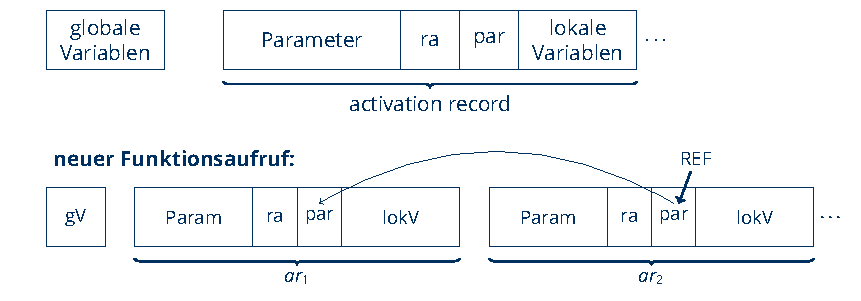
\includegraphics[width=\textwidth]{tut11-abb}
	
	\pause
	
	\textbf{Funktionsaufrufe übersetzen:}
	\begin{itemize}
		\item Parameter \texttt{LOAD} \& \texttt{PUSH}
		\item Funktion \texttt{CALL}
	\end{itemize}

\end{frame}

\begin{frame} \frametitle{Befehlssemantik der $AM_1$}
	\footnotesize
	\begin{minipage}{\dimexpr0.4\linewidth-\fboxrule-\fboxsep}
		$b \in \{ \text{global}, \text{lokal}\}$ \\
		$r$ \dots aktueller REF
	\end{minipage}
	\begin{minipage}{\dimexpr0.6\linewidth-\fboxrule-\fboxsep}
		\begin{equation*}
			adr(r,b,o) = \begin{cases}
			r+o & \text{wenn } b = \text{lokal} \\
			o & \text{wenn } b = \text{global}
			\end{cases}
		\end{equation*}
	\end{minipage}

	\pause
	
	\begin{tabular}{p{2cm} p{\dimexpr\linewidth-\fboxrule-\fboxsep-2cm}}
		\emph{Befehl} & \emph{Auswirkungen}  \\ \hline
		LOAD($b$,$o$) & Lädt den Inhalt von Adresse $adr(r,b,o)$ auf den Datenkeller, inkrementiere Befehlszähler \\
		STORE($b$,$o$) & Speichere oberstes Datenkellerelement an $adr(r,b,o)$, inkrementiere Befehlszähler \\
		WRITE($b$,$o$) & Schreibe Inhalt an Adresse $adr(r,b,o)$ auf das
		Ausgabeband, inkrementiere Befehlszähler \\
		READ($b$,$o$) & Lies oberstes Element vom Eingabeband, speichere
		an Adresse $adr(r,b,o)$, inkrementiere Befehlszähler \\
	\end{tabular}
\end{frame}

\begin{frame} \frametitle{Befehlssemantik der $AM_1$}
	\scriptsize		
	\begin{tabular}{p{2cm} p{\dimexpr\linewidth-\fboxrule-\fboxsep-2cm}}
		\emph{Befehl} & \emph{Auswirkungen}  \\ \hline
		LOADI($o$) & Ermittle Wert ($=b$) an Adresse $r+o$, Lade Inhalt
		von Adresse $b$ auf Datenkeller, inkrementiere Befehlszähler \\
		STOREI($o$) & Ermittle Wert ($=b$) an Adresse $r+o$, nimm
		oberstes Datenkellerelement, speichere dieses an
		Adresse $b$, inkrementiere Befehlszähler \\
		WRITEI($o$) & Ermittle Wert ($=b$) an Adresse $r+o$, schreibe den
		Inhalt an Adresse $b$ auf Ausgabeband, inkrementiere Befehlszähler \\
		READI($o$) & Ermittle Wert ($=b$) an Adresse $r+o$, lies das oberste
		Element vom Eingabeband, speichere es an Adresse $b$ , inkrementiere Befehlszähler \\
		LOADA($b$,$o$) & Lege $adr(r,b,o)$ auf Datenkeller, inkrementiere Befehlszähler \\			
		PUSH & oberstes Element vom Datenkeller auf Laufzeitkeller, Befehlszähler inkrementieren \\
		CALL $adr$ & Befehlszählerwert inkrementieren und auf LZK legen, Befehlszähler auf $adr$ setzen, REF auf LZK legen, REF auf Länge des LZK ändern \\
		INIT $n$ & $n$-mal $0$ auf den Laufzeitkeller legen \\
		RET $n$ & im LZK alles nach REF-Zeiger löschen, oberstes Element des LZK als REF setzen, oberstes Element des LZK als Befehlszähler setzen, $n$ Elemente von LZK löschen
	\end{tabular}
\end{frame}

\begin{frame} \frametitle{Merkhilfen}
	\footnotesize
	\textbf{Übersetzen:}
	\begin{itemize}
		\item \texttt{*x} wird mit \texttt{I}-Befehlen übersetzt (außer in Funktionsköpfen)
		\item \texttt{\&x} wird mit \texttt{A}-Befehlen übersetzt
		\item \texttt{BEFEHL}($global$, $o$) verhält sich wie in der AM${}_\text{0}$
		\item \texttt{BEFEHL}($lokal$, $o$) verhält sich ähnlich wie in der AM${}_\text{0}$ mit \textit{Adressberechnung} ($r+o$) vorher
	\end{itemize}

	\pause 
	
	\textbf{Ablaufprotokolle:}
	\begin{itemize}
		\item \texttt{I}-Befehle: Wert-an-Adresse-Prozess zweimal machen
		\item \texttt{A}-Befehle: Adresse direkt verarbeiten (nicht erst Wert auslesen)
	\end{itemize}
\end{frame}

\section{Übungsblatt 11}

\begin{frame}[fragile] \frametitle{Aufgabe 1 -- Teil (a)}
	\footnotesize
	\textbf{Aufgabe.} 
	Gegeben ist folgender $AM_1$-Code:  
	
	\begin{minipage}{\dimexpr0.33\linewidth-\fboxrule-\fboxsep}
		\begin{lstlisting}[style=am0]
INIT 1;
CALL 18;
INIT 0;
LOAD(lokal,-2);
LIT 0;
GT;
JMC 17;
LIT 2;
LOADI(-3);
		\end{lstlisting}
	\end{minipage}
	\begin{minipage}{\dimexpr0.33\linewidth-\fboxrule-\fboxsep}
		\begin{lstlisting}[style=am0, firstnumber=10]
MUL;
STOREI(-3);
LOAD(lokal,-2);
LIT 1;
SUB;
STORE(lokal,-2);
JMP 4;
RET 2;
INIT 0;
		\end{lstlisting}
	\end{minipage}
	\begin{minipage}{\dimexpr0.33\linewidth-\fboxrule-\fboxsep}
		\begin{lstlisting}[style=am0, firstnumber=19]
READ(global,1);
LOADA(global,1);
PUSH;
LOAD(global,1);
PUSH;
CALL 3;
WRITE(global,1);
JMP 0;
		\end{lstlisting}
	\end{minipage}
	
	\bigskip
	
	Führen Sie $12$ Schritte der $AM_1$ auf der Konfiguration $\sigma = (22, \epsilon, 1:3:0:1, 3, \epsilon, \epsilon)$ aus.
\end{frame}


\begin{frame} \frametitle{Aufgabe 1 -- Teil (a)}
	\footnotesize
	\textbf{Lösung.}
	
	\scriptsize
	\begin{center}
		\begin{tabu}{rccrclcccrcrl}
			\head & BZ && DK && LZK && REF && Inp && Out & \\ \hline 
			( & 22 &,& $\epsilon$ &,& 1:3:0:1 &,& 3 &,& $\epsilon$ &,& $\epsilon$ & ) \\
			( & 23 &,& 1 &,& 1:3:0:1 &,& 3 &,& $\epsilon$ &,& $\epsilon$ & ) \\
			( & 24 &,& $\epsilon$ &,& 1:3:0:1:1 &,& 3 &,& $\epsilon$ &,& $\epsilon$ & ) \\
			( & 3 &,& $\epsilon$ &,& 1:3:0:1:1:25:3 &,& 7 &,& $\epsilon$ &,& $\epsilon$ & ) \\
			( & 4 &,& $\epsilon$ &,& 1:3:0:1:1:25:3 &,& 7 &,& $\epsilon$ &,& $\epsilon$ & ) \\
			( & 5 &,& 1 &,& 1:3:0:1:1:25:3 &,& 7 &,& $\epsilon$ &,& $\epsilon$ & ) \\
			( & 6 &,& 0:1 &,& 1:3:0:1:1:25:3 &,& 7 &,& $\epsilon$ &,& $\epsilon$ & ) \\
			( & 7 &,& 1 &,& 1:3:0:1:1:25:3 &,& 7 &,& $\epsilon$ &,& $\epsilon$ & ) \\
			( & 8 &,& $\epsilon$ &,& 1:3:0:1:1:25:3 &,& 7 &,& $\epsilon$ &,& $\epsilon$ & ) \\
			( & 9 &,& 2 &,& 1:3:0:1:1:25:3 &,& 7 &,& $\epsilon$ &,& $\epsilon$ & ) \\
			( & 10 &,& 1:2 &,& 1:3:0:1:1:25:3 &,& 7 &,& $\epsilon$ &,& $\epsilon$ & ) \\
			( & 11 &,& 2 &,& 1:3:0:1:1:25:3 &,& 7 &,& $\epsilon$ &,& $\epsilon$ & ) \\
			( & 12 &,& $\epsilon$ &,& 2:3:0:1:1:25:3 &,& 7 &,& $\epsilon$ &,& $\epsilon$ & ) \\
			\hline
			( & 13 &,& 1 &,& 2:3:0:1:1:25:3 &,& 7 &,& $\epsilon$ &,& $\epsilon$ & ) \\
			( & 14 &,& 1:1 &,& 2:3:0:1:1:25:3 &,& 7 &,& $\epsilon$ &,& $\epsilon$ & ) \\
		\end{tabu}
	\end{center}
\end{frame}


\begin{frame} \frametitle{Aufgabe 1 -- Teil (b)}
	\scriptsize
	
	\textbf{Symboltabellen:}	
	\begin{align*}
		%		\text{tab}_{\texttt{f}} &= [ \texttt{f}/(\text{proc}, 1), \texttt{a}/(\text{var}, \text{lokal}, -3), \texttt{b}/(\text{var-ref}, -2) ] \\
		\text{lokal-tab}_{\texttt{f}} &= [ \texttt{f}/(\text{proc}, 1), \texttt{a}/(\text{var}, \text{lokal}, -3), \texttt{b}/(\text{var-ref}, -2), \texttt{c}/(\text{var}, \text{lokal}, 1) ] \\
		\text{lokal-tab}_{\texttt{main}} &= [ \texttt{f}/(\text{proc}, 1), \texttt{b}/(\text{var}, \text{global}, 1), \texttt{a}/(\text{var}, \text{lokal}, 1) ]
	\end{align*}

	\textbf{Übersetzung:}
	
	\adjustbox{valign=t}{%
	\begin{minipage}{\dimexpr0.33\linewidth-\fboxrule-\fboxsep}
		\begin{tabular}{>{\ttfamily}r >{\ttfamily}l}
			& INIT 1; \\
			& CALL 2; \\
			& JMP 0; \\
			\\
			\textcolor{cdgray!50}{\tiny 1} & INIT 1; \\
			& LOAD(lokal, -3); \\
			& STORE(lokal, 1); \\
		\end{tabular}
	\end{minipage}}
	\adjustbox{valign=t}{%
	\begin{minipage}{\dimexpr0.33\linewidth-\fboxrule-\fboxsep}
		\begin{tabular}{>{\ttfamily}r >{\ttfamily}l}
			\textcolor{cdgray!50}{\tiny 1.2.1} & LOAD(lokal, 1); \\
			& LIT 0; \\
			& GT; \\
			& JMC 1.2.2; \\
			& LOADI(-2); \\
			& LIT 2; \\
			& MUL; \\
			& STOREI(-2); \\
			& LOAD(lokal, 1); \\
			& LIT 1; \\
			& SUB; \\
			& STORE(lokal, 1); \\
			& JMP 1.2.1; \\
			\textcolor{cdgray!50}{\tiny 1.2.2} & RET 2; \\
		\end{tabular}
	\end{minipage} }
	\adjustbox{valign=t}{%
	\begin{minipage}{\dimexpr0.33\linewidth-\fboxrule-\fboxsep}
		\begin{tabular}{>{\ttfamily}r >{\ttfamily}l}
			\textcolor{cdgray!50}{\tiny 2} & INIT 1; \\
			& READ(lokal, 1); \\
			& LIT 1; \\
			& STORE(global, 1); \\
			& LOAD(lokal, 1); \\
			& PUSH; \\
			& LOADA(global, 1); \\
			& PUSH; \\
			& CALL 1; \\
			& WRITE(global, 1); \\
			& RET 0; \\
		\end{tabular}
	\end{minipage} }
\end{frame}







%%%%%%%%%%%%%%%%%%%%%%%%%%%%%%%%%%%%%%%%%%%%%%%%%%%%%%%%%%%%%%%%%%%%%%%%%%%%%%%%%

\begin{frame}[fragile] \frametitle{Aufgabe 2 -- Teil (a)}
	\footnotesize
	\textbf{Aufgabe.}
	\begin{lstlisting}
#include <stdio.h>
int x, y;
void f(...) {...}
void g(int a, int *b) {
	int c;
	c = 3;
	if (c == *b) while (a > 0) f(&a, b);
}
void main () {...}
	\end{lstlisting}
	
	Übersetzen Sie die Sequenz der Statements im Rumpf von \texttt{g} in entsprechenden AM${}_\text{1}$-Code mit baumstrukturierten Adressen (mittels \textit{stseqtrans}). Sie brauchen keine Zwischenschritte anzugeben. Geben Sie zunächst die benötigte Symboltabelle $tab_{\texttt{g}}$ an.
\end{frame}


\begin{frame} \frametitle{Aufgabe 2 -- Teil (a)}
	\footnotesize
	\textbf{Lösung.}
	
	\begin{align*}
		tab_{\texttt{g}} = [ \enskip &\texttt{f}/(proc, 1), \texttt{g}/(proc, 2),\\
		&\texttt{x}/(var, global, 1), \texttt{y}/(var, global, 2), \\
		&\texttt{a}/(var, lokal, -3), \texttt{b}(var-ref, -2), \texttt{c}/(var, lokal, 1) \enskip]
	\end{align*}
	
	\pause
	
	\begin{tabular}{>{\ttfamily}r >{\ttfamily}l >{\ttfamily}l >{\ttfamily}l >{\ttfamily}l >{\ttfamily}l}
		& LIT 3; STORE(lokal,1); \\
		& LOAD(lokal,1); LOADI (-2); EQ; JMC 2.2.1; \\
		2.2.2.1: & LOAD(lokal,-3); LIT 0; GT; JMC 2.2.2.2; \\
		& LOADA(lokal,-3); PUSH; \\
		& LOAD(lokal,-2); PUSH; CALL 1; \\
		& JMP 2.2.2.1; \\
		2.2.2.2: & 2.2.1:
	\end{tabular}
\end{frame}

\begin{frame}[fragile] \frametitle{Aufgabe 2 -- Teil (b)}
	\footnotesize
	\textbf{Aufgabe.}
	
	\begin{minipage}{\dimexpr0.33\linewidth-\fboxrule-\fboxsep}
		\begin{lstlisting}[style=am0]
INIT 1;
CALL 13;
INIT 0;
LOADI (-2);
LIT 2;
GT;
JMC 12;
		\end{lstlisting}
	\end{minipage}
	\begin{minipage}{\dimexpr0.33\linewidth-\fboxrule-\fboxsep}
		\begin{lstlisting}[style=am0, firstnumber=8]
LOADI (-2);
LIT 2;
DIV;
STOREI (-2);
RET 1;
INIT 0;
READ(global , 1);
		\end{lstlisting}
	\end{minipage}
	\begin{minipage}{\dimexpr0.33\linewidth-\fboxrule-\fboxsep}
		\begin{lstlisting}[style=am0, firstnumber=15]
LOADA(global , 1);
PUSH;
CALL 3;
WRITE(global , 1);
JMP 0;
		\end{lstlisting}
	\end{minipage}
	
	\bigskip
	
	Erstellen Sie ein Ablaufprotokoll der AM${}_\text{1}$, indem Sie sie schrittweise ablaufen lassen, bis die Maschine terminiert. Die Anfangskonfiguration sei $(14, \epsilon, 0 : 0 : 1, 3, 4, \epsilon)$. Sie müssen nur Zellen ausfüllen, deren Wert sich im Vergleich zur letzten Zeile geändert hat.
\end{frame}

\begin{frame} \frametitle{Aufgabe 2 -- Teil (b)}
	\footnotesize
	\textbf{Lösung.}
	\scriptsize
	\begin{center}
		\begin{tabu}{rrcrclcccrcrl}
			\head & BZ && DK && LZK && REF && Inp && Out & \\ \hline
			( & 14 &,& $\epsilon$ &,& 0:0:1 &,& 3 &,& 4 &,& $\epsilon$ & ) \\
			( & 15 &,& $\epsilon$ &,& 4:0:1 &,& 3 &,& $\epsilon$ &,& $\epsilon$ & ) \\
			( & 16 &,& 1 &,& 4:0:1 &,& 3 &,& $\epsilon$ &,& $\epsilon$ & ) \\
			( & 17 &,& $\epsilon$ &,& 4:0:1:1 &,& 3 &,& $\epsilon$ &,& $\epsilon$ & ) \\
			( & 3 &,& $\epsilon$ &,& 4:0:1:1:18:3 &,& 6 &,& $\epsilon$ &,& $\epsilon$ & ) \\
			( & 4 &,& $\epsilon$ &,& 4:0:1:1:18:3 &,& 6 &,& $\epsilon$ &,& $\epsilon$ & ) \\
			( & 5 &,& 4 &,& 4:0:1:1:18:3 &,& 6 &,& $\epsilon$ &,& $\epsilon$ & ) \\
			( & 6 &,& 2:4 &,& 4:0:1:1:18:3 &,& 6 &,& $\epsilon$ &,& $\epsilon$ & ) \\
			( & 7 &,& 1 &,& 4:0:1:1:18:3 &,& 6 &,& $\epsilon$ &,& $\epsilon$ & ) \\
			( & 8 &,& $\epsilon$ &,& 4:0:1:1:18:3 &,& 6 &,& $\epsilon$ &,& $\epsilon$ & ) \\
			( & 9 &,& 4 &,& 4:0:1:1:18:3 &,& 6 &,& $\epsilon$ &,& $\epsilon$ & ) \\
			( & 10 &,& 2:4 &,& 4:0:1:1:18:3 &,& 6 &,& $\epsilon$ &,& $\epsilon$ & ) \\
			( & 11 &,& 2 &,& 4:0:1:1:18:3 &,& 6 &,& $\epsilon$ &,& $\epsilon$ & ) \\
			( & 12 &,& $\epsilon$ &,& 2:0:1:1:18:3 &,& 6 &,& $\epsilon$ &,& $\epsilon$ & ) \\
			( & 18 &,& $\epsilon$ &,& 2:0:1 &,& 3 &,& $\epsilon$ &,& $\epsilon$ & ) \\
			( & 19 &,& $\epsilon$ &,& 2:0:1 &,& 3 &,& $\epsilon$ &,& 2 & ) \\
			( & 0 &,& $\epsilon$ &,& 2:0:1 &,& 3 &,& $\epsilon$ &,& 2 & ) \\
		\end{tabu}
	\end{center}
\end{frame}

\end{document}

